\documentclass[manuscript]{copernicus}
\usepackage{graphicx}
\usepackage{subcaption}
%\usepackage{subfigure}
\graphicspath{{pictures/}}          % graphics
\renewcommand{\thefigure}{S\arabic{figure}}
\renewcommand{\thetable}{S\arabic{table}}

\begin{document}
\clearpage
\setcounter{page}{1}
%%%%%%%%%%%%%%%%%%%%%%%%%%%%%
\section*{Supplement}
\subsection*{S.1 Aerodynamical resistance}
\begin{equation}
  \Psi_m(\zeta) =
  \begin{cases}
   \log(\frac{1+x^2}{2}\cdot(\frac{1+x}{2})^2) - 2\cdot \arctan(x+\frac{\pi}{2}) & \quad \emph{if} \quad -2 < \zeta < 0,\\
   - \beta \cdot \zeta & \quad \emph{if} \quad \zeta \ge 0.
  \end{cases}
  \label{eq:psim}
\end{equation}
\begin{equation}
  \Psi_h(\zeta) =
  \begin{cases}
   2\cdot\log(\frac{1+x^2}{2}) & \quad \emph{if} \quad -2 < \zeta < 0,\\
   - \beta \cdot \zeta & \quad \emph{if} \quad \zeta \ge 0.
  \end{cases}
  \label{eq:psih}
\end{equation}
$x = (1-\gamma\cdot\zeta)^\frac{1}{4}$, $\beta = 4.7$, $\gamma = 15$ (from Kansas experiment).
%\begin{table}[!htbp]
%  \caption{Molecular diffusivity for a gas $i$ given as ration $D_\chem{H_2O}/D_i$, reactivity $f^i_0$, and effective Henry's Law constant $H^i_*$.}
%  \begin{tabular}{lcrr@{$\cdot$}l}
%    \tophline
%    & $D_\chem{H_2O}/D_i$ & $f^i_0$ & \multicolumn{2}{l}{$H^i_*$}\\
%    & & & \multicolumn{2}{l}{(\unit{M\,atm^{-1}})}\\
%    \middlehline
%    \chem{O_3}     & 1.6 & 1.0 & 1 & $10^{-2}$\\
%    \chem{SO_2}    & 1.9 & 0.0 & 1 & $10^5$\\
%    \chem{NO_2}    & 1.6 & 0.1 & 1 & $10^{-2}$\\
%    \chem{H_2O_2}  & 1.4 & 1.0 & 1 & $10^5$\\
%    \chem{HCHO}    & 1.3 & 0.0 & 6 & $10^3$\\
%    \chem{NO}      & 1.3 & 0.0 & 2 & $10^{-3}$\\
%    \chem{CH_3CHO} & 1.6 & 15.0 & \multicolumn{2}{l}{$0$}\\
%    \bottomhline
%  \end{tabular}
  %\belowtable{} % Table Footnotes
%\end{table}
%%%%%%%%%%%%%%%%%%%%%%%%%%%%%
\subsection*{S.2 Dynamic viscosity of air and quasi-laminar resistance}
\begin{figure}[!htbp]
  \centering
  \includegraphics[height=0.4\textheight]{pictures/dynamic_viscosity.pdf}
  \caption{Sutherland's law and divergence linear fits with one or two degrees of freedom. The fit $\mu(T) = m\cdot T$ is implemented in the Oslo~CTM3. Despite its strong divergence at lower and higher temperatures, the impact of this choice on the results is negligible.}
\end{figure}
%
\begin{figure}[!htbp]
  \centering
  \includegraphics[height=0.4\textheight]{pictures/dynamic_viscosity_zo_Rb.pdf}
  \caption{Comparison of resulting $z_o$ and $R_b$ for $\mu(T) = m\cdot T$  (left panel) and Sutherland's law (right panel). The example displays the distributions for \chem{H_2O} after one day of model integration for both, rough and calm sea case.}
\end{figure}

\begin{figure}[!htbp]
  \centering
  \begin{subfigure}[b]{1.\textwidth}
    \includegraphics[height=0.45\textheight]{pictures/dynamic_viscosity_Rbi_1.pdf}
    \caption{}
  \end{subfigure}
  \\
  \begin{subfigure}[b]{1.\textwidth}
    \includegraphics[height=0.45\textheight]{pictures/dynamic_viscosity_Rbi_2.pdf}
    \caption{}
  \end{subfigure}
  \caption{Resulting $R_b$ for different species. Shown are results of one day model integrations for both, Sutherland's law and $\mu(T) = m\cdot T$. Shown are also the percentages above / below the given threshold.}
\end{figure}
\clearpage
%%%%%%%%%%%%%%%%%%%%%%%%%%%%%
%\subsection*{S.3 Stomatal conductance}
%\begin{table*}[!htbp]
%  \caption{Tabulated parameters for stomatal conductance computation in the EMEP scheme}
%  \begin{tabular}{lcccccccccccccc}
%    \tophline
%    Code$^*$ & $g_\text{max}$ & $f_\text{min}$ & $\phi_a$ & $\phi_b$ & $\phi_c$ & $\phi_d$ & $\phi_e$ & $\phi_f$ & $\phi_\text{AS}$ & $\phi_\text{AE}$ & $\alpha_\text{light}$ & $T_\text{min}$ & $T_\text{opt}$ & $T_\text{max}$ \\
%    & (\unit{mmol\,s^{-1}\,m^{-2}}) &&&&&&(\unit{days})&(\unit{days})&(\unit{days})&(\unit{days})&&(\unit{^\circ C})&(\unit{^\circ C})&(\unit{^\circ C})\\
%    \middlehline
%    CF & 140 & 0.1 & 0.8 & 0.8 & 0.8 & 0.8 & 1 & 1 & 0 & 0 & 0.006 & 0 & 18 & 36  \\
%    DF & 150 & 0.1 & 0 & 0 & 1 & 0 & 20 & 30 & 0 & 0 & 0.006 & 0 & 20 & 35  \\
%    NF & 200 & 0.1 & 1 & 1 & 0.2 & 1 & 130 & 60 & 80 & 35 & 0.013 & 8 & 25 & 38 \\
%    BF & 200 & 0.02 & 1 & 1 & 0.3 & 1 & 130 & 60 & 80 & 35 & 0.009 & 1 & 23 & 39 \\
%    TC & 300 & 0.1 & 0.1 & 1 & 0.1 & 0 & 45 & 0 & 0 & 0.0105 & 0.01 & 12 & 26 & 40 \\
%    MC & 300 & 0.019 & 0.1 & 0.1 & 1 & 0.1 & 0 & 45 & 0 & 0 & 0.0048 & 0 & 25 & 51  \\
%    RC & 360 & 0.02 & 0.2 & 0.2 & 1 & 0.2 & 20 & 45 & 0 & 0 & 0.0023 & 8 & 24 & 50  \\
%    SNL & 60 & 0.01 & 1 & 1 & 1 & 1 & 1 & 1 & 0 & 0 & 0.009 & 1 & 18 & 36 \\
%    GR & 270 & 0.01 & 1 & 1 & 1 & 1 & 0 & 0 & 0 & 0 & 0.009 & 12 & 26 & 40 \\
%    MS & 200 & 0.01 & 1 & 1 & 0.2 & 1 & 130 & 60 & 80 & 35 & 0.012 & 4 & 20 & 37 \\
%    WE & 0 & 1 & 1 & 1 & 1 & 1 & 1 & 1 & 1 & 1 & 1 & 0 & 1 & 0 \\
%    TU & 0 & 1 & 1 & 1 & 1 & 1 & 1 & 1 & 1 & 1 & 1 & 0 & 1 & 0  \\
%    DE & 0 & 1 & 1 & 1 & 1 & 1 & 1 & 1 & 1 & 1 & 1 & 0 & 1 & 0  \\
%    W & 0 & 1 & 1 & 1 & 1 & 1 & 1 & 1 & 1 & 1 & 1 & 0 & 1 & 0 \\
%    ICE & 0 & 1 & 1 & 1 & 1 & 1 & 1 & 1 & 1 & 1 & 1 & 0 & 1 & 0 \\
%    U & 0 & 1 & 1 & 1 & 1 & 1 & 1 & 1 & 1 & 1 & 1 & 0 & 1 & 0 \\
%    \bottomhline
%  \end{tabular}
%  \\
%  \vspace{2\baselineskip}
%  \begin{tabular}{lcccccccccc}
%    \tophline
%    Code$^*$ & $D_\text{max}$ & $D_\text{min}$ & $D_\text{crit}$ & $R_\chem{SO}$ & $R_\chem{O_3}$ & $h$ & $d_\text{SGS}$ & $d_\text{EGS}$ & $\nabla d_\text{SGS}$ & $\nabla d_\text{EGS}$\\% & $\text{LAI}_\text{min}$ & $\text{LAI}_\text{max}$ & LS & LE \\
%    &(\unit{kPA})&(\unit{kPa})&(\unit{kPa})&(\unit{s\,m^{-1}})&(\unit{s\,m^{-1}})&(\unit{m})&(\unit{day})&(\unit{day})&(\unit{days/^\circ lat})&(\unit{days/^\circ lat})\\%&(\unit{m^2\,m^{-2}})&(\unit{m^2\,m^{-2}})&(\unit{days})&(\unit{days}) \\
%    \middlehline
%    CF & 0.5 & 3 & 1000 & 0 & 200 & 20 & 0 & 366 & 0 & 0\\% & 5 & 5 & 1 & 1\\
%    DF & 1 & 3.25 & 1000 & 0 & 200 & 20 & 100 & 307 & 1.5 & -2.0 \\%& 0 & 4 & 20 & 30\\
%    NF & 1 & 3.2 & 1000 & 0 & 200 & 8 & 0 & 366 & 0 & 0\\% & 4 & 4 & 1 & 1\\
%    BF & 2.2 & 4 & 1000 & 0 & 200 & 15 & 0 & 366 & 0 & 0 \\%& 4 & 4 & 1 & 1\\
%    TC & 1.2 & 3.2 & 8 & 0 & 200 & 1 & 123 & 213 & 2.57 & 2.57\\% & 0 & 3.5 & 70 & 20\\
%    MC & 1 & 2.5 & 1000 & 0 & 200 & 2 & 123 & 237 & 2.57 & 2.57\\% & 0 & 3 & 70 & 44\\
%    RC & 0.31 & 2.7 & 10 & 0 & 200 & 1 & 130 & 250 & 0 & 0\\% & 0 & 4.2 & 35 & 65\\
%    SNL & 1.3 & 3 & 1000 & 0 & 400 & 0.5 & 0 & 366 & 0 & 0\\% & 2 & 3 & 192 & 96\\
%    GR & 1.3 & 3 & 1000 & 0 & 1000 & 0.3 & 0 & 366 & 0 & 0\\% & 2 & 3.5 & 140 & 135\\
%    MS & 1.3 & 3.2 & 1000 & 0 & 200 & 2 & 0 & 366 & 0 & 0\\% & 2.5 & 2.5 & 1 & 1\\
%    WE  & 1 & 0 & 1000 & 50 & 400 & 0.5 & 0 & 366 & 0 & 0\\% & 0 & 0 & 0 & 0\\
%    TU & 1 & 0 & 1000 & 500 & 400 & 0.5 & 0 & 366 & 0 & 0\\% & 0 & 0 & 0 & 0\\
%    DE & 1 & 0 & 1000 & 1000 & 2000 & 0 & 0 & 366 & 0 & 0\\% & 0 & 0 & 0 & 0\\
%    W  & 1 & 0 & 1000 & 1 & 2000 & 0 & 0 & 366 & 0 & 0\\% & 0 & 0 & 0 & 0\\
%    ICE & 1 & 0 & 1000 & 1000 & 2000 & 0 & 0 & 366 & 0 & 0\\% & 0 & 0 & 0 & 0\\
%    U & 1 & 0 & 1000 & 400 & 400 & 10 & 0 & 366 & 0 & 0\\% & 0 & 0 & 0 & 0\\
%    \bottomhline
%  \end{tabular}
%  \belowtable{$^*$: CF -- temperate/boreal coniferous; DF -- temperate/boreal deciduous; NF -- Mediterranean needleleaf; BF -- Mediterranean broadleaf; TC -- temperate crop; MC -- Mediterranean crop; RC -- root crop; SNL -- moorland; GR -- grass; MS -- Mediterranean shrub; WE -- wetlands; TU -- tundra; DE -- desert; W -- water; ICE -- ice.}
%\end{table*}

%\clearpage
\subsection*{S.3 Latitude dependent vegetation height}
\begin{figure}[!htbp]
  \centering
  \includegraphics[height=0.4\textheight]{pictures/tree_height.pdf}
  \caption{Extension of the latitude dependent vegetation height from northern hemisphere mid latitudes only to a global description. Example heights are shown for coniferous (CF), deciduous (DF), needleleaf (NF), and broadleaf (BF) forests as well as Mediterranean shrub (MS). As reference the original range of EMEP is added.}
\end{figure}

\subsection*{S.4 Temperature dependent greening season (python 2.7)}
{\scriptsize
\begin{verbatim}
#----------------------------------------------------------------------------------
import numpy as np
import pandas as pd
import xarray as xr
#----------------------------------------------------------------------------------
def start_growing_season_fixed(lat, **kwargs):
    '''
    Begin of growing season parameterization adapted from SMOKE-BEIS.
    '''
    bLeap = kwargs.pop('leap', False)
    if (bLeap):
       MAY31 = 152
       NOV1  = 306
       DEC31 = 366
    else:
       MAY31 = 151
       NOV1  = 305
       DEC31 = 365
    
    if lat < -65:
        return((0,))
    elif lat < -23:
        return((NOV1,1))
    elif lat <= 23:
        return((1,))
    elif lat < 65:
        return(((lat-23)*4.5,))
    else:
        return((0,))
#----------------------------------------------------------------------------------
def end_growing_season_fixed(lat, **kwargs):
    '''
    End of growing season parameterization adapted from SMOKE-BEIS.
    '''
    bLeap = kwargs.pop('leap', False)
    if (bLeap):
       MAY31 = 152
       NOV1  = 306
       DEC31 = 366
    else:
       MAY31 = 151
       NOV1  = 305
       DEC31 = 365
       
    if lat < -65:
        return((0,))
    elif lat < -23:
        return((DEC31,MAY31))
    elif lat <= 23:
        return((DEC31,))
    elif lat < 65:
        return((DEC31-(lat-23)*3.3,))
    else:
        return((0,))
#----------------------------------------------------------------------------------
def growing_season(temperature,**kwargs):
    '''
    Agricultural rule of thumb definition of growing season:
    5 consecutive days above 5 degree Celsius 
    and vice versa for end of growing season.
    '''
    # Shift start day of evaluation.
    s_shift = kwargs.pop('s_shift',365/2)
    # Number of days that need to fulfill temperature criteria
    degree_days_crit = kwargs.pop('ddc', 5)
    # Temperature criteria
    temperature_crit = kwargs.pop('tc', 5)
    # Switch to southern hemisphere evaluation
    sh = kwargs.pop('sh', False)
    # Activate verbose
    verbose = kwargs.pop('verbose', False)
    # Counters
    count_gdd = 0
    count_days = 0
    start_gs = (0,False)
    end_gs = (0,False)
    
    if sh:
    # Shift the temperature by halve a year - shifted back later.
        temp = temperature.roll(time=s_shift)
    else:
        temp = temperature
    for itemp in temp:
        count_days += 1
        if not start_gs[1]:
            if itemp > temperature_crit:
                count_gdd += 1
            else:
                count_gdd = 0
            if count_gdd == degree_days_crit:
                if sh:
                    start_gs = (count_days+s_shift, True)
                else:
                    start_gs = (count_days, True)
                count_gdd = 0
        elif start_gs[1] and not end_gs[1] and count_days>s_shift:
            if itemp <= temperature_crit:
                count_gdd += 1
                if verbose:
                    print(count_days, count_gdd)
            else:
                count_gdd = 0
            if count_gdd == degree_days_crit:
                if sh:
                    end_gs = (count_days-s_shift, True)
                else:
                    end_gs = (count_days, True)
                count_gdd = 0
       
    return({'sgs':start_gs,'egs':end_gs})
#----------------------------------------------------------------------------------
def growing_season_stadyn(xr_temp):
    '''
    Preprocess the greening season for OsloCTM3.
    Setting using the 5deg-5days criteria and in case this fails
    or is out of the defined bounds,
    fall back to SMOKE-BEIS parameterization.
    '''
    # Fetch leap year from input data
    bLeap = False
    if xr_temp.time.size==366:
       bLeap = True
    # Use 5deg-5days criteria   
    if (xr_temp.lat > 45 and xr_temp.lat < 85):
        gs = growing_season(xr_temp)
        sgs = (gs['sgs'][0],)
        egs = (gs['egs'][0],)
        if ( not gs['sgs'][1] or not gs['egs'][1] or sgs[0]>=egs[0]):
            # Check for failing 5deg-5days criteria => Fall back to fixed
            sgs = start_growing_season_fixed(xr_temp.lat.data, leap=bLeap)
            egs = end_growing_season_fixed(xr_temp.lat.data, leap=bLeap)
    elif (xr_temp.lat < -35 and xr_temp.lat >= -65):
        gs = growing_season(xr_temp, sh=True)
        sgs = (gs['sgs'][0],1)
        egs = (xr_temp.size, gs['egs'][0])
        # Check for failing 5deg-5days criteria => Fall back to fixed
        if (not gs['sgs'][1] or not gs['egs'][1] or sgs[0]>=egs[0]):
            sgs = start_growing_season_fixed(xr_temp.lat.data, leap=bLeap)
            egs = end_growing_season_fixed(xr_temp.lat.data, leap=bLeap)
    # Use SMOKE-BEIS parameterization
    else:
        sgs = start_growing_season_fixed(xr_temp.lat.data, leap=bLeap)
        egs = end_growing_season_fixed(xr_temp.lat.data, leap=bLeap)
    # Generate GDAY and GLEN fields
    # in case no growing season has been allocated
    if (sgs[0]==egs[0]==0):
        gday = np.repeat(0,len(xr_temp.time))
        glen = 0
    # in normal cases
    else:
        # handle northern hemisphere
        if len(sgs)==1:
            gday = np.concatenate((np.repeat(0,int(sgs[0])-1),
                                   np.arange(1,int(egs[0])-int(sgs[0])+1),
                                   np.repeat(0,len(xr_temp.time)-
                                   int(egs[0])+1)))
            glen = int(egs[0])-int(sgs[0])+1
        # handle southern hemisphere
        else:
            gday = np.concatenate((np.arange(1,int(egs[1])+1)+len(xr_temp.time)
                                   -int(sgs[0])+1,
                                   np.repeat(0,int(sgs[0])-int(egs[1])),
                                   np.arange(1,len(xr_temp.time)-int(sgs[0])+1)))
            glen = len(xr_temp.time)-(int(sgs[0])-int(egs[1]))+1
    # This should not happen, but in case it does, print info.
    if not(len(gday)==len(xr_temp.time)):
        print(xr_temp, sgs, egs)
    # Output
    data_gday = xr.DataArray(gday.astype(int),[('time', xr_temp.time.data)])
    return(data_gday, (int)(glen))
#----------------------------------------------------------------------------------
\end{verbatim}
}
\clearpage

\subsection*{S.5 De-accumulation of photosynthetic active radiation (PAR) from OpenIFS}
\begin{figure}[!htbp]
  \centering
  \includegraphics[height=0.4\textheight, clip, trim={0.7cm 0.7cm 0.7cm 0.65cm}]{pictures/PAR_as_is.png}
  \caption{Example output from OpenIFS for January 2nd 2005. PAR is accumulated over the period of one day.}
\end{figure}

\begin{figure}[!htbp]
  \centering
  \includegraphics[height=0.4\textheight, clip, trim={0.7cm 0.7cm 0.7cm 0.65cm}]{pictures/PAR_partly_deaccumulated.png}
  \caption{Partly de-accumulated output from OpenIFS. $\text{PPFD}(t_i) = \text{PAR}(t_{i+1})-\text{PAR}(t_i)$.}
\end{figure}

\begin{figure}[!htbp]
  \centering
  \includegraphics[height=0.4\textheight, clip, trim={0.75cm 0.75cm 0.75cm 0.65cm}]{pictures/PAR_deaccumulating_00h.png}
  \caption{De-accumulation of $t=00\,\unit{UTC}$ in the partly de-accumulated fields. $\text{PPFD}(t=00\,\unit{UTC}) = \text{PAR}(t=00\,\unit{UTC}) - \left[\text{PAR}(t=21\,\unit{UTC}-1\,\unit{day})-\text{PAR}(t=12\,\unit{UTC}-1\,\unit{day})\right]$.}
\end{figure}
%\clearpage

\subsection*{S.6 Normalized zonal average ozone dry deposition velocity}
\begin{figure}[!htbp]
  \centering
  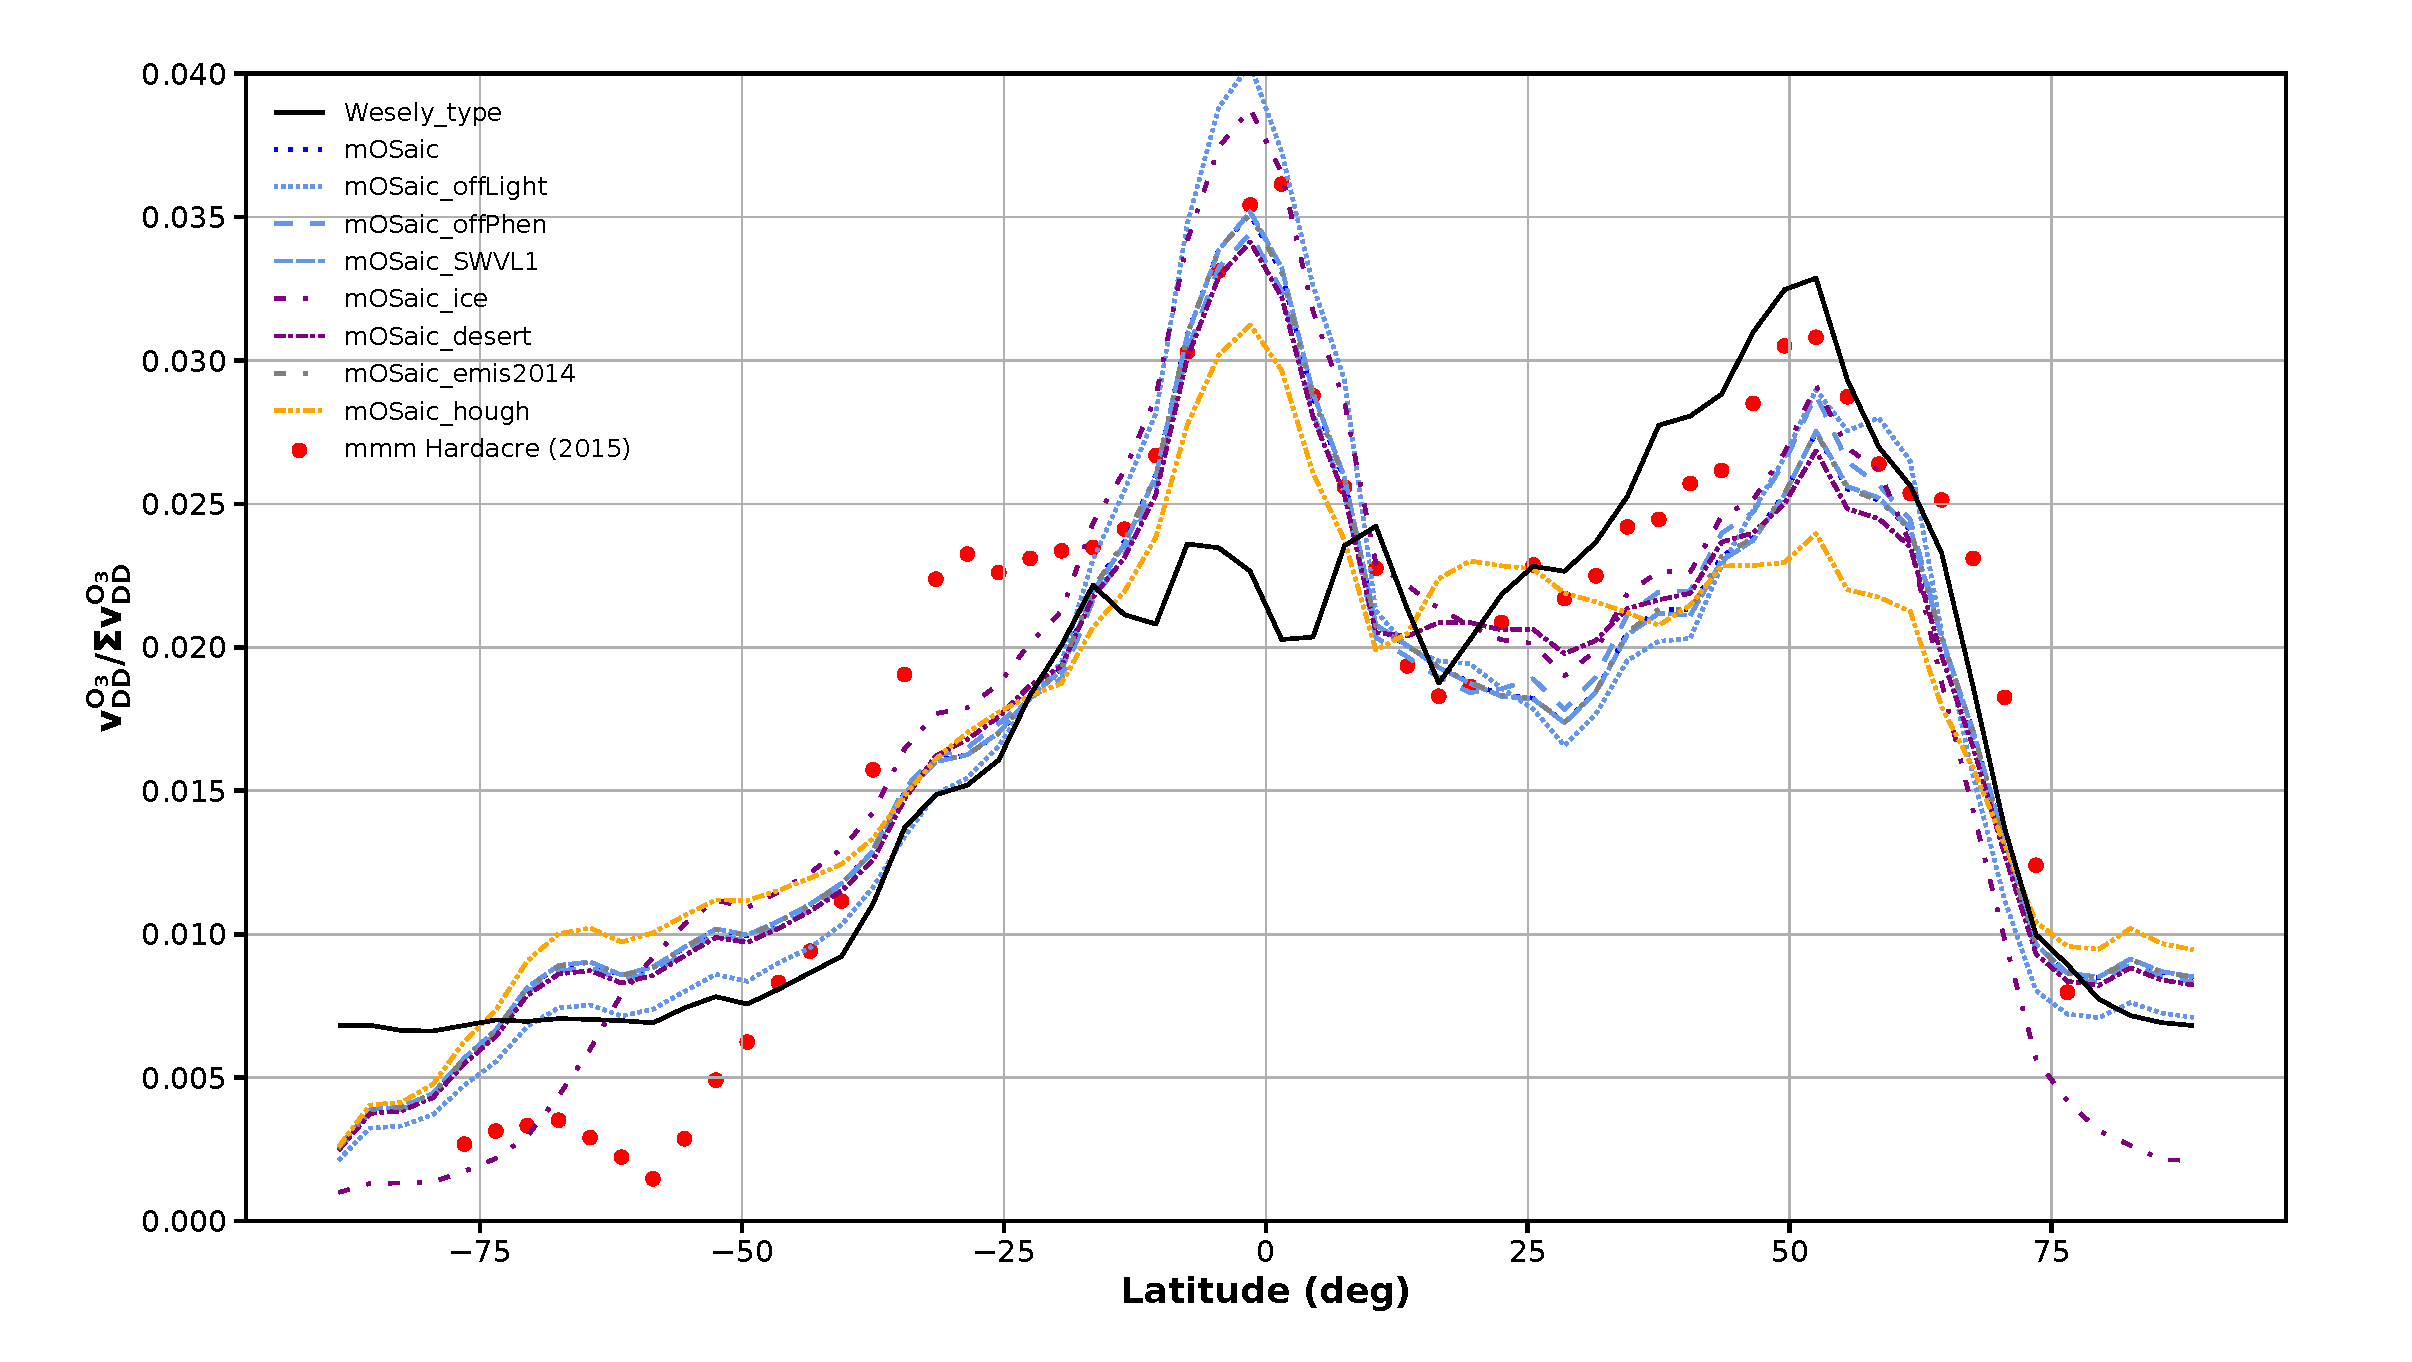
\includegraphics[height=0.4\textheight, clip, trim={0.7cm 0.7cm 0.7cm 0.55cm}]{pictures/final-norm_total_ozone_drydepvelo_v2}
  \caption{Normalized zonal average ozone dry deposition velocity.}
\end{figure}

\subsection*{S.7 Surface resistance of ozone}
\begin{table*}[!htbp]
  \caption{Surface resistance of ozone $R^\chem{O_3}$ adapted from  Wesely (1989); Hough (1991): $^*$ CF -- temperate/boreal coniferous; DF -- temperate/boreal deciduous; NF -- Mediterranean needleleaf; BF -- Mediterranean broadleaf; TC -- temperate crop; MC -- Mediterranean crop; RC -- root crop; SNL -- moorland; GR -- grass; MS -- Mediterranean shrub; WE -- wetlands; TU -- tundra; DE -- desert; W -- water; ICE -- ice.}
  \begin{tabular}{lc}
    \tophline
    Code$^*$ & $R_\chem{O_3}$\\
         & (\unit{s\,m^{-1}})\\
    \middlehline
    CF, DF, NF, BF &  1000\\
    TC &  200 \\
    SNL, WE, U & 400 \\
    GR, MS  & 1000 \\
    TU, DE  & 385 \\
    W, ICE  & 1430 \\
    \bottomhline
 \end{tabular}
  %\belowtable{}
\end{table*}

\subsection{S.8 Comparison with MACC-reanalysis}
\begin{figure}[!htbp]
  \centering
  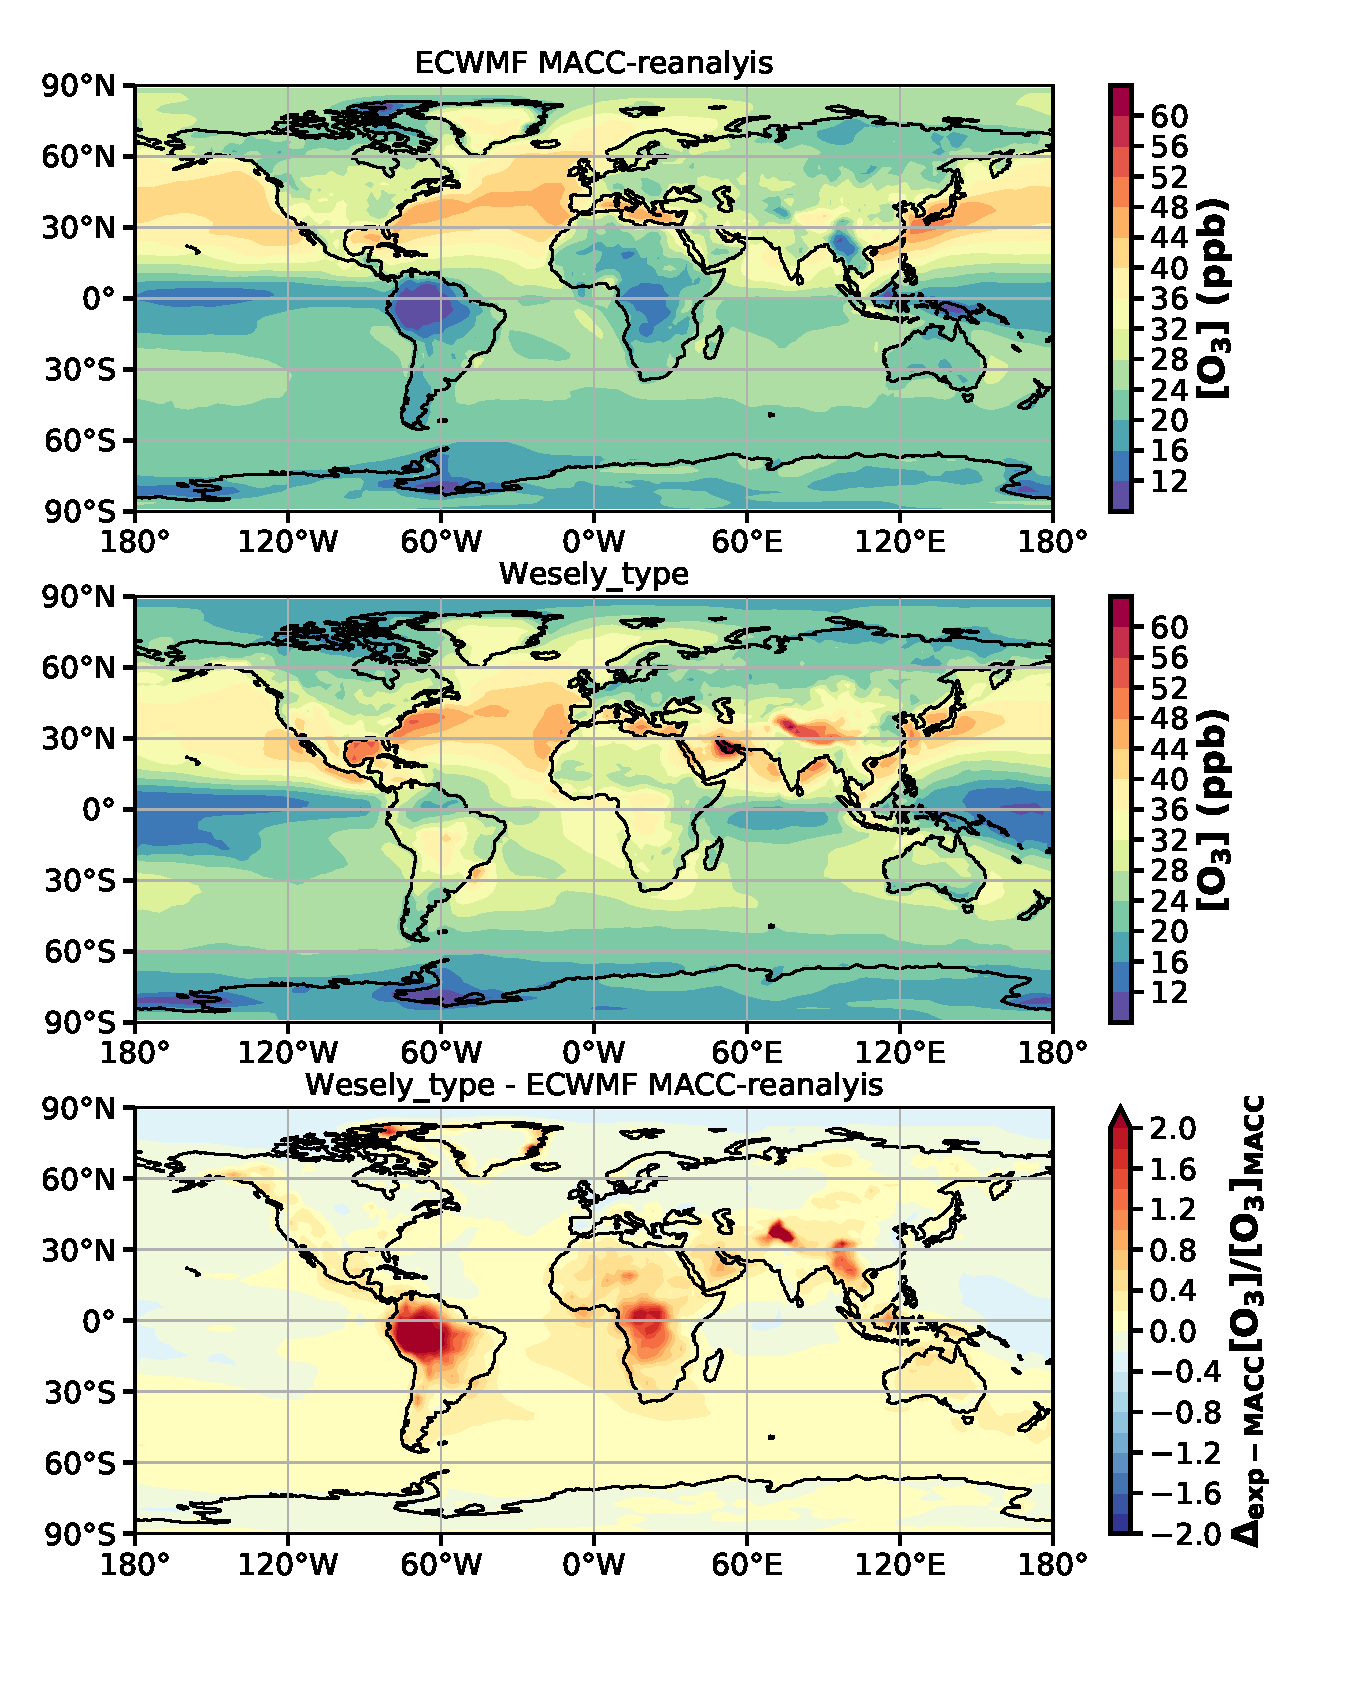
\includegraphics[height=0.5\textheight, clip, trim={0.7cm 0.7cm 0.7cm 0.55cm}]{pictures/annual_mean_surface_ozone_2005_Wesely_type}
  \caption{Mean ozone concentrations for the year 2005. (a) MACC-reanalysis (surface); (b) Oslo~CTM3 \emph{Wesely\_type} (lowermost model level); (c) Relative difference.}
\end{figure}

\end{document}
